\section{Данные}

\subsection{Котировки драгоценных металлов}

Основным источником рыночных данных служит MOEX ISS API~---
открытый интерфейс Московской биржи.
Загружаются дневные OHLCV-данные (цены открытия, максимума, минимума, закрытия
и объём торгов) для четырёх инструментов:

\begin{itemize}
    \item \textbf{GLDRUB\_TOM}~--- золото в рублях, данные с 9 января 2018 г.,
          2\,031 торговый день;
    \item \textbf{SLVRUB\_TOM}~--- серебро в рублях, данные с 9 января 2018 г.,
          1\,926 торговых дней;
    \item \textbf{PLTRUB\_TOM}~--- платина в рублях, данные с 22 октября 2024 г.,
          346 торговых дней;
    \item \textbf{PLDRUB\_TOM}~--- палладий в рублях, данные с 22 октября 2024 г.,
          346 торговых дней.
\end{itemize}

Ввиду ограниченности исторических данных по платине и палладию
основной акцент в эмпирическом анализе делается на золоте и серебре.

\subsection{Реализованная волатильность}

Поскольку внутридневные тиковые данные недоступны, реализованная
волатильность считается по дневным OHLC-ценам с помощью range-based
оценщиков~\cite{Garman1980, Parkinson1980}. Они точнее обычного
оценщика по ценам закрытия (Close-to-Close), так как используют ещё
максимум и минимум дня.

\textbf{Оценщик Garman--Klass}~\cite{Garman1980} (используется как основной):
\begin{equation}\label{eq:gk}
    \widehat{\sigma}^2_t = \tfrac{1}{2}\bigl(\ln H_t - \ln L_t\bigr)^2
    - \bigl(2\ln 2 - 1\bigr)\bigl(\ln C_t - \ln O_t\bigr)^2,
\end{equation}
где $O_t, H_t, L_t, C_t$~--- цены открытия, максимума, минимума и закрытия в день $t$.
Эффективность оценщика~\eqref{eq:gk} примерно в 7{,}4 раза выше, чем у Close-to-Close.

\textbf{Оценщик Parkinson}~\cite{Parkinson1980}:
\begin{equation}\label{eq:park}
    \widehat{\sigma}^2_t = \frac{\bigl(\ln H_t - \ln L_t\bigr)^2}{4 \ln 2}.
\end{equation}

Аннуализированная волатильность вычисляется как
$\widehat{\sigma}^{\mathrm{ann}}_t = \sqrt{252 \cdot \widehat{\sigma}^2_t}$.
Описательные статистики для основных инструментов приведены в таблице~\ref{tab:rv_stats}.

\begin{table}[h!]
\centering
\caption{Описательные статистики аннуализированной волатильности (оценщик Garman--Klass)}
\label{tab:rv_stats}
\begin{tabular}{lrrrrrr}
\hline
Инструмент & $N$ & Среднее & Медиана & Станд.\ откл. & Минимум & Максимум \\
\hline
GLDRUB\_TOM & 1\,931 & 0{,}156 & 0{,}115 & 0{,}166 & 0{,}001 & 1{,}659 \\
SLVRUB\_TOM & 1\,635 & 0{,}276 & 0{,}196 & 0{,}270 & 0{,}001 & 2{,}317 \\
\hline
\end{tabular}
\end{table}

На рисунке~\ref{fig:rv_timeseries} представлена динамика аннуализированной
реализованной волатильности обоих инструментов за весь период наблюдений.
Вертикальная пунктирная линия отмечает 24 февраля 2022~г.~---
момент резкого скачка волатильности, образующего структурный разрыв в ряду.

\begin{figure}[H]
\centering
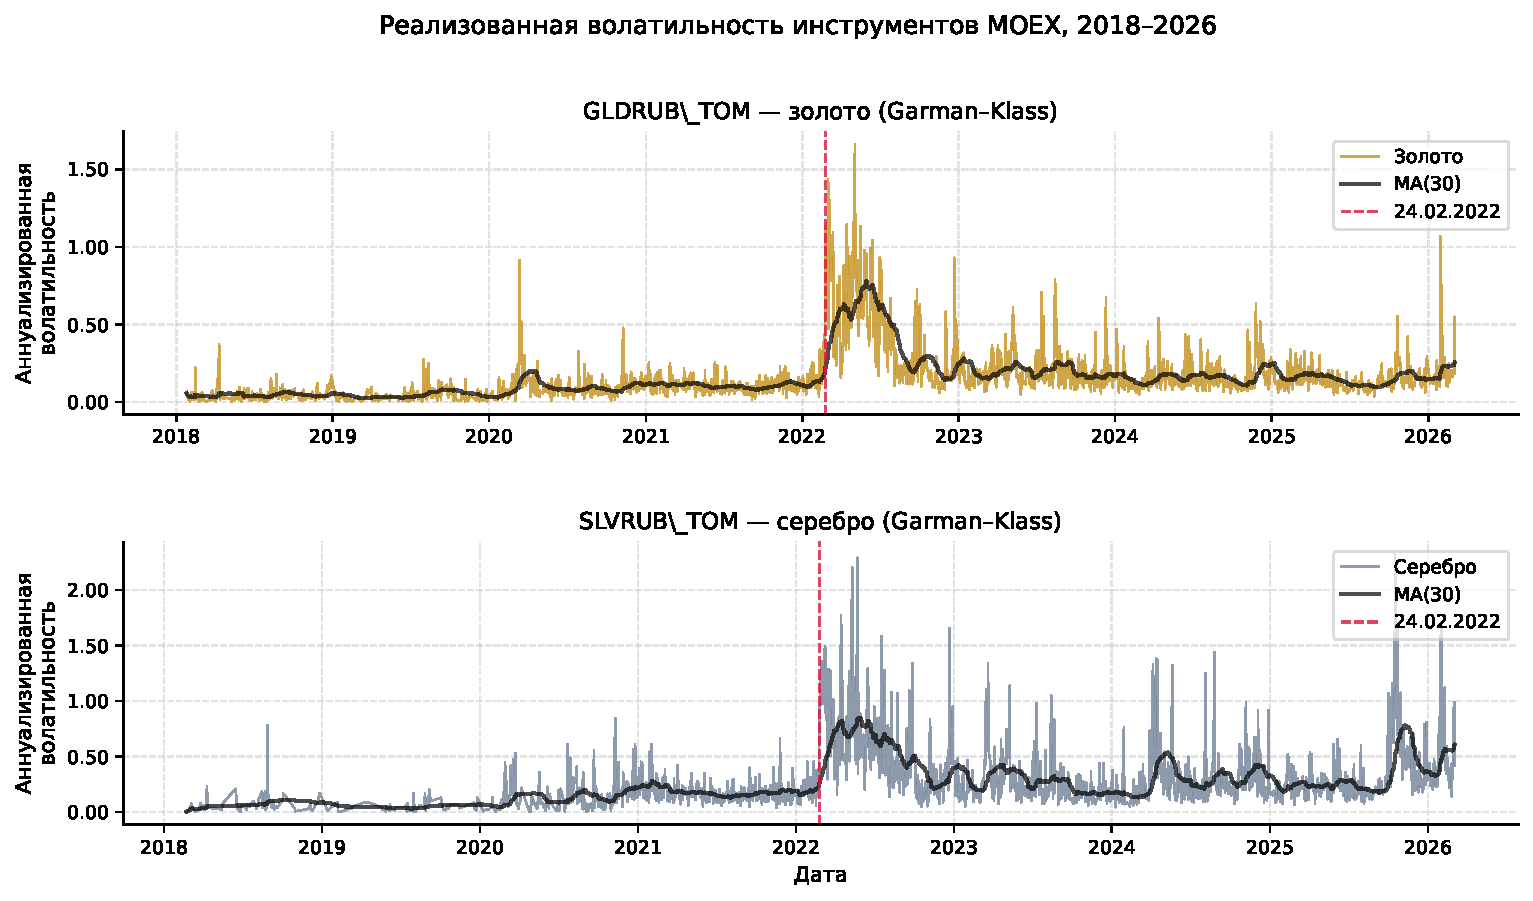
\includegraphics[width=\linewidth]{figures/rv_timeseries.pdf}
\caption{Реализованная волатильность GLDRUB\_TOM (золото) и SLVRUB\_TOM (серебро),
         оценщик Garman--Klass, 2018--2026.
         Жирная линия~--- скользящее среднее MA(30).
         Пунктир~--- 24.02.2022.}
\label{fig:rv_timeseries}
\end{figure}

\subsection{Sentiment и attention признаки}

\subsubsection{Новостной поток (RSS)}

Парсер RSS-лент собирает статьи из шести источников:
Коммерсантъ, Ведомости, Интерфакс, ТАСС, РБК и Investing.com.
Фильтрация осуществляется по ключевым словам, связанным с металлами,
макроэкономикой и геополитикой (54 ключевых слова).
Статьи хранятся в \texttt{data/sentiment/rss\_news.csv}.

\subsubsection{Telegram-каналы}

Для получения sentiment розничных инвесторов и профессиональных аналитиков
используется Telegram API (Telethon).
Парсятся 12 активных русскоязычных каналов финансовой тематики:
\textit{@russianmacro}, \textit{@bcs\_express}, \textit{@cbrstocks},
\textit{@markettwits}, \textit{@economika}, \textit{@banksta},
\textit{@alfawealth}, \textit{@investiciiotpraktika} и др.
Фильтрация по ключевым словам (металлы, курсы, ставки, макро).
Собрано 23\,733 релевантных сообщений за период 2018--2026 (2\,028 дней).
Дневной score вычисляется как взвешенное по просмотрам среднее
лексического sentiment; среднее значение --- $+0{,}194$.
Данные хранятся в \texttt{data/sentiment/telegram\_sentiment.csv}.

\subsubsection{GDELT}

GDELT (Global Database of Events, Language, and Tone)~--- открытая база данных,
индексирующая мировой новостной поток каждые 15 минут.
Используется компонент GKG (Global Knowledge Graph),
предоставляющий агрегированные оценки тональности (Tone) новостей по темам.
Загружены данные за период 2018--2026 гг.\ (718 дней с ненулевым покрытием
по интересующим темам), среднее количество релевантных записей~--- 100--150 в день.
В дни без прямого покрытия применяется forward fill.

\subsubsection{Google Trends}

Индекс поисковой активности Google Trends отражает относительный интерес
пользователей к теме за период и служит прямой мерой внимания инвесторов~\cite{Da2011}.
Загружены данные по трём группам запросов:
\textit{metals\_ru} (<<золото цена>>, <<купить золото>>, <<серебро цена>> и др.),
\textit{macro\_ru} (<<ключевая ставка>>, <<инфляция россия>>, <<курс доллара>> и др.),
\textit{metals\_en} (<<gold price>>, <<silver price>> и др.)
за период 2018--2026 гг.\ (3\,043 дня), регион~--- Россия.

\subsubsection{Макроэкономические индикаторы}

С XML API Банка России загружены:
официальные курсы USD/RUB, EUR/RUB и CNY/RUB (ежедневно, 3\,060 наблюдений)
и история ключевой ставки (решения ЦБ РФ с 2018 г.).
Через FRED API дополнительно загружены:
цена нефти Brent (DCOILBRENTEU, 2\,121 наблюдение, среднее \$73{,}66/барр.),
индекс доллара США (DTWEXBGS, 2\,094 наблюдения, среднее 118{,}18),
индекс волатильности VIX (VIXCLS, 2\,140 наблюдений, среднее 19{,}65),
ставка ФРС (FEDFUNDS) и CPI США (CPIAUCSL).

\subsubsection{Объёмы торгов MOEX}

Дневные объёмы торгов по каждому инструменту выступают в роли прокси
внимания инвесторов. Нормализация осуществляется через 30-дневный
скользящий z-score с последующим применением sigmoid-функции:
$\mathrm{attention\_volume}_t = \sigma(z_t) \in [0, 1]$.

\subsection{Итоговый датасет}

Все источники объединяются агрегатором в файл \texttt{daily\_sentiment.csv}
с дневной частотой за период 2018-01-01~--- 2026-05-28 (3\,070 дней, 25 признаков).
Итоговый вектор включает:
sentiment-признаки (RSS, GDELT, Telegram, комбинированный),
attention-признаки (Google Trends, объёмы MOEX),
макроэкономику ЦБ РФ (USD/RUB, EUR/RUB, CNY/RUB, ключевая ставка)
и макроэкономику FRED (Brent, DXY, VIX, CPI США, ставка ФРС и их лог-доходности).
Доля заполненных значений по всем признакам~--- 100\%.
Пропущенные значения заполняются методом forward fill для числовых рядов
и нулями для sentiment-переменных в периоды отсутствия данных.

Рисунок~\ref{fig:sentiment_dynamics} демонстрирует динамику ключевых
sentiment- и attention-индексов за 2018--2026~гг.
Заметно резкое ухудшение комбинированного sentiment в феврале--марте 2022~г.
и всплеск внимания инвесторов (Google Trends) в период санкционного шока,
что подтверждает информационную ценность добавленных источников.

\begin{figure}[H]
\centering
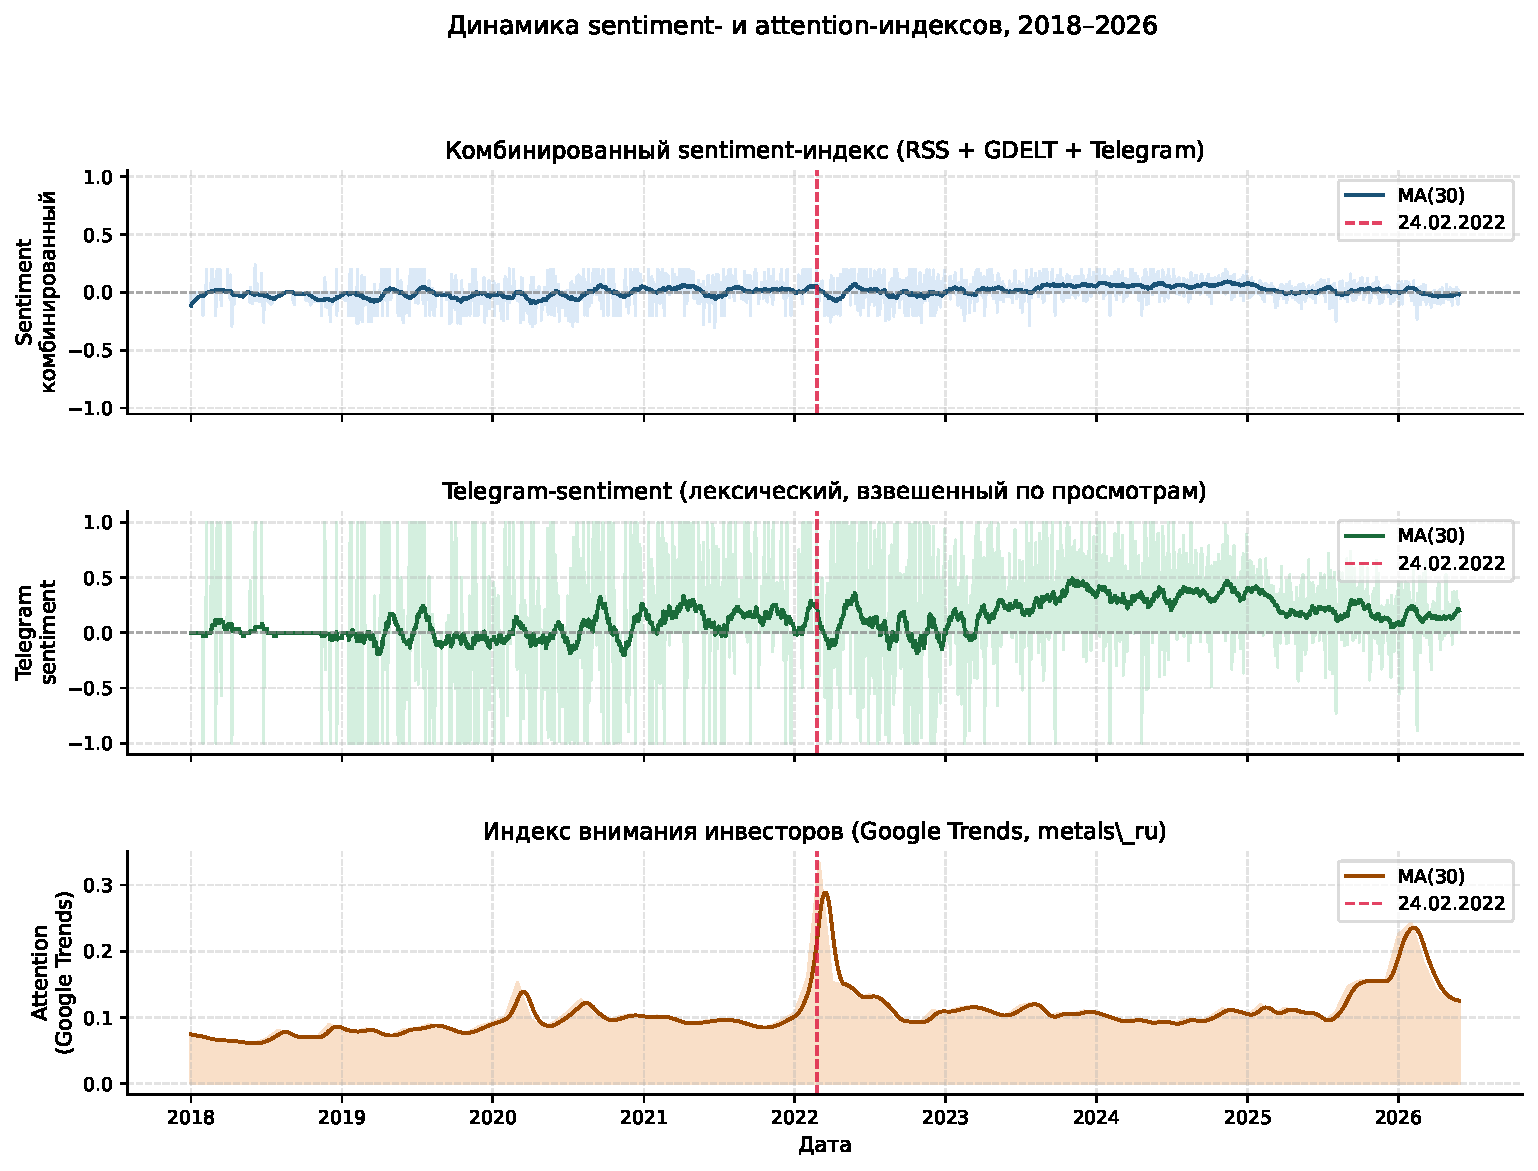
\includegraphics[width=\linewidth]{figures/sentiment_dynamics.pdf}
\caption{Динамика sentiment- и attention-индексов, 2018--2026.
         Сверху вниз: комбинированный sentiment (RSS+GDELT+Telegram),
         Telegram-sentiment, индекс внимания Google Trends (metals\_ru).
         Жирная линия~--- MA(30). Красный пунктир~--- 24.02.2022.}
\label{fig:sentiment_dynamics}
\end{figure}
